%
% tikztemplate.tex -- template for standalon tikz images
%
% (c) 2019 Prof Dr Andreas Müller, Hochschule Rapperswil
%
\documentclass[tikz]{standalone}
\usepackage{amsmath}
\usepackage{times}
\usepackage{txfonts}
\usepackage{pgfplots}
\usepackage{csvsimple}
\usetikzlibrary{arrows,intersections,math}
\begin{document}
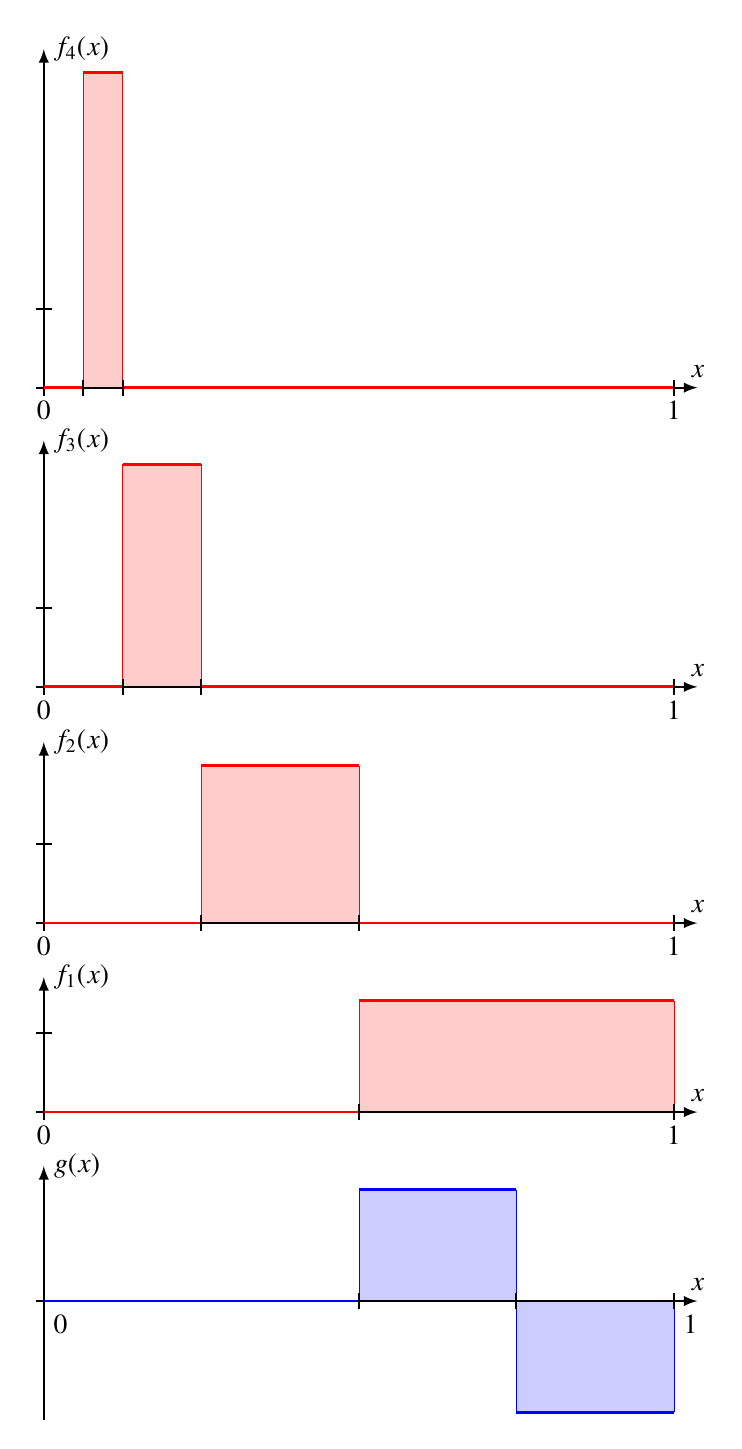
\begin{tikzpicture}[>=latex]

\def\a{1}
\def\d{2}

\def\fkurve#1#2{
\pgfmathparse{\a*sqrt(2)}
\xdef\a{\pgfmathresult}
\pgfmathparse{\d/2}
\xdef\d{\pgfmathresult}
\begin{scope}[yshift=#1]
\fill[color=red!20] ({8*\d/2},0)--({8*\d},0)--({8*\d},\a)--({8*\d/2},\a)--cycle;

\draw[->,line width=0.7pt] (-0.1,0)--(8.3,0) coordinate[label=$x$];
\draw[->,line width=0.7pt] (0,-0.1)--(0,{\a+0.3}) coordinate[label={right:$f_{#2}(x)$}];


\draw[color=red,line width=1pt] (0,0)--({8*\d/2},0);
\draw[color=red,line width=0.1pt] ({8*\d/2},0)--({8*\d/2},\a);
\draw[color=red,line width=1pt] ({8*\d/2},\a)--({8*\d},\a);
\draw[color=red,line width=0.1pt] ({8*\d},\a)--({8*\d},0);
\draw[color=red,line width=1pt] ({8*\d},0)--({8*1},0);

\draw[line width=0.7pt] (-0.1,1)--(0.1,1);
\draw[line width=0.7pt] ({8*1},-0.1)--({8*1},0.1);
\draw[line width=0.7pt] ({8*\d},-0.1)--({8*\d},0.1);
\draw[line width=0.7pt] ({4*\d},-0.1)--({4*\d},0.1);

\node at (8,-0.05) [below] {$1$};
\node at (0,-0.05) [below] {$0$};
\end{scope}
}

\fkurve{0cm}{1}
\fkurve{2.4cm}{2}
\fkurve{5.4cm}{3}
\fkurve{9.2cm}{4}

\begin{scope}[yshift=-2.4cm]
\fill[color=blue!20] (4,0)--(6,0)--(6,{sqrt(2)})--(4,{sqrt(2)})--cycle;
\fill[color=blue!20] (8,0)--(6,0)--(6,{-sqrt(2)})--(8,{-sqrt(2)})--cycle;
\draw[->,line width=0.7pt] (-0.1,0)--(8.3,0) coordinate[label=$x$];
\draw[->,line width=0.7pt] (0,{-sqrt(2)-0.1})--(0,{sqrt(2)+0.3}) coordinate[label={right:$g(x)$}];;
\draw[line width=1pt,color=blue] (0,0)--(4,0);
\draw[line width=0.1pt,color=blue] (4,0)--(4,{sqrt(2)});
\draw[line width=1pt,color=blue] (4,{sqrt(2)})--(6,{sqrt(2)});
\draw[line width=0.1pt,color=blue] (6,{sqrt(2)})--(6,{-sqrt(2)});
\draw[line width=1pt,color=blue] (6,{-sqrt(2)})--(8,{-sqrt(2)});
\draw[line width=0.1pt,color=blue] (8,{-sqrt(2)})--(8,0);
\draw[line width=0.7pt] (4,-0.1)--(4,0.1);
\draw[line width=0.7pt] (6,-0.1)--(6,0.1);
\draw[line width=0.7pt] (8,-0.1)--(8,0.1);
\node at (8,-0.05) [below right] {$1$};
\node at (0,-0.05) [below right] {$0$};
\end{scope}

\end{tikzpicture}
\end{document}

